\section{Conclusion and Plan for the Graduation Project (HK262)}
\label{ch:plan}

\subsection{Conclusion}

This report presented the first phase of the project ``Design of an E-Learning System with AI Integration'': a university-grade e-learning platform in the style of BKeL. We analyzed the needs of lecturers and students, specified seven use cases, and designed a three-tier architecture and a fourteen-table relational schema in third normal form. The most important design contributions are the fifteen-session model of a class, the capacity trigger with row locking, the composite foreign key that keeps quiz telemetry consistent with the skill of its question, and a PIN attendance protocol with expiry, rate limiting, constant-time comparison and one record per student and session.

The implementation consists of a typed Express API with authentication, role checks and the attendance transaction, and a Next.js prototype that reproduces the BKeL visual identity with a light and a dark theme. A pilot dataset for CO2003 provides fifteen sessions and forty skill-labeled questions. The report also states the current gaps: the front end is not connected to the API, tests are not automated, and several secondary flows (manual attendance, question authoring, session editing) are missing.

\subsection{Direction Given by the Supervisor}

After the third meeting, the supervisor asked the team to finish the e-learning system properly before extending it. The plan below follows this direction: the first eight weeks bring the system to a complete, tested state; only then are the intelligent features of the full project added, and they remain optional for the evaluation of the system itself.

\subsection{Plan for Weeks 1--15 of the Graduation Project (HK262)}

Table~\ref{tab:plan} lists the week-by-week plan. The plan is organized in five phases with a deliverable at the end of each phase. Figure~\ref{fig:gantt} gives an overview.

\begin{longtblr}[caption={Week-by-week plan for HK262}, label={tab:plan}]{colspec={Q[l,1.3cm]X[l]X[l]}, row{1}={font=\bfseries}, hline{1,Z}={0.8pt}, hline{2}={0.4pt}, rowsep=2pt, rows={font=\small}}
Week & Tasks & Deliverable\\
1 & Review feedback on this report; freeze scope of phase~1; write an OpenAPI description of all endpoints; set up Docker Compose (PostgreSQL, API, front end) & API specification; one-command local environment\\
2 & Connect login, registration and the course list to the API; replace demonstration data by API data; error and loading states & Working login and course list on real data\\
3 & Connect sessions, timetable and enrollment; bulk session creation from the lecturer screen; room-conflict check & Schedule module end to end\\
4 & Connect PIN attendance (open, close, check-in) and statistics; add the live list refresh; manual marking and PIN regeneration & Attendance module end to end; feature freeze of phase~1\\
5 & Question authoring (UC3): create, edit, delete questions with skill labels; import of the CO2003 bank into the database; bilingual questions & Question bank module\\
6 & Automated tests: SQL constraint tests, API tests for every endpoint and role, concurrency tests (enrollment, PIN attempts) & Test suite in continuous integration\\
7 & Security review against the OWASP verification checklist; rate limit on login; password reset flow; audit of error messages & Security review report\\
8 & Performance measurement of the main endpoints with 60 and 300 simulated students; indexes tuned from query plans & Measured results for NFR6\\
9 & Design of the learning-support extension: student competency view built from quiz history (UC4); definition of skill model and data export from \code{quiz_interactions} & Design document of the extension\\
10 & Implementation of a first baseline for per-skill mastery estimation from quiz history, with a fallback to empirical accuracy & Baseline estimator service\\
11 & Integration of the estimator into the student view; recommendations of sessions to review; expansion of the question bank to 3--5 questions per skill & Competency view in the course page\\
12 & Usability study with 8--10 students and 2 lecturers: tasks, observation, SUS questionnaire~\cite{brooke1996sus} & Study protocol; raw data\\
13 & Analysis of the study; fixes of the most serious problems; accessibility check with WCAG 2.1 criteria~\cite{wcag21} & Study report; fixed issues\\
14 & Deployment on a test server (HTTPS, environment variables, backups); user guide and administrator guide & Deployed system; manuals\\
15 & Final report, slides and demonstration; rehearsal of the defense & Final report; defense package\\
\end{longtblr}

\begin{figure}[H]
\centering
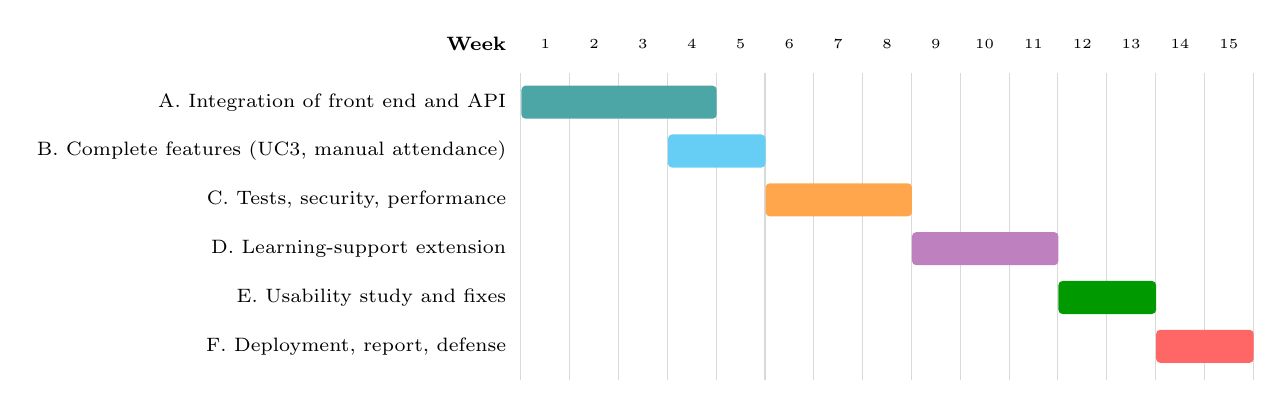
\begin{tikzpicture}[x=0.62cm, y=0.62cm,
    bar/.style={rectangle, rounded corners=1.5pt, minimum height=0.42cm, inner sep=0pt},
    >=stealth]
\foreach \w in {1,...,15} {
    \node[font=\tiny] at (\w-0.5+4.2,0.6) {\w};
    \draw[gray!30] (\w+4.2,0) -- (\w+4.2,-6.3);
}
\draw[gray!30] (4.2,0) -- (4.2,-6.3);
\node[font=\scriptsize\bfseries, anchor=east] at (4.1,0.6) {Week};
\def\rowitem#1#2#3#4#5{%
  \node[font=\scriptsize, anchor=east] at (4.1,-#1) {#2};
  \node[bar, fill=#5, anchor=west, minimum width={(#4-#3+1)*0.62cm}] at (#3+3.2,-#1) {};}
\rowitem{0.6}{A. Integration of front end and API}{1}{4}{teal!70}
\rowitem{1.6}{B. Complete features (UC3, manual attendance)}{4}{5}{cyan!60}
\rowitem{2.6}{C. Tests, security, performance}{6}{8}{orange!70}
\rowitem{3.6}{D. Learning-support extension}{9}{11}{violet!50}
\rowitem{4.6}{E. Usability study and fixes}{12}{13}{green!60!black}
\rowitem{5.6}{F. Deployment, report, defense}{14}{15}{red!60}
\end{tikzpicture}
\caption{Overview of the plan for HK262 (weeks 1--15)}
\label{fig:gantt}
\end{figure}

\subsection{Planned Meetings and Report Milestones}

Meetings with the supervisor are held every two weeks, with an optional Friday afternoon session on request. The milestones for the report of the current semester are 15 November 2026 (at least 30 pages), 30 November 2026 (at least 50 pages) and 15 December 2026 (at least 70 pages). The final defense is on 31 December 2026.

\subsection{Intelligent Learning Support: Background for Weeks 9--11}

The extension of weeks 9--11 builds on the field of knowledge tracing, which models the knowledge state of a learner from the sequence of answers. The classical model, Bayesian Knowledge Tracing, estimates for each skill the probability that the learner has mastered it~\cite{corbett1995knowledge}; neural variants, introduced with Deep Knowledge Tracing, predict the probability of a correct answer from the whole sequence~\cite{piech2015deep}. The data model of the first phase already stores what these methods need: one row per answer with the user, the skill, the correctness and the time. The decision about which model to use will be taken in week~9 after reviewing the amount of data that can be collected; with a small number of students, a simple and interpretable baseline is more appropriate than a neural model. This part is explicitly separated from the evaluation of the e-learning system itself.
